\documentclass{article}
\usepackage{tikz}
\usepackage{geometry}
\geometry{
paperheight=108mm,paperwidth=192mm,
total={152mm,68mm},
left=20mm,
top=20mm,
}
\usepackage{fontspec}
\usepackage{xcolor}
\setmainfont{CascadiaMono.ttf}
\pagenumbering{gobble}
\pagecolor{black}
\hyphenpenalty 10000
\exhyphenpenalty 10000
\begin{document}
\noindent \textcolor{white}
{Hallo World}

\begin{tikzpicture}
\draw[color=cyan, very thick] (0mm,0mm)--(5mm,5mm);
\end{tikzpicture}

\begin{tikzpicture}
\draw[color=cyan, very thick] (0mm,5mm)--(5mm,0mm);
\end{tikzpicture}
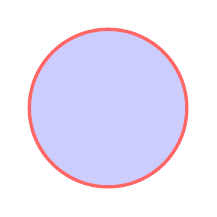
\begin{tikzpicture}
\filldraw[color=red!60, fill=blue!20, very thick](10mm,10mm) circle (10mm);
\end{tikzpicture}
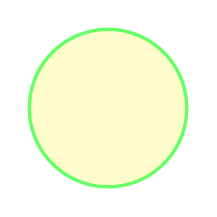
\begin{tikzpicture}
\filldraw[color=green!60, fill=yellow!20, very thick](10mm,10mm) circle (10mm);
\end{tikzpicture}
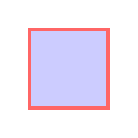
\begin{tikzpicture}
\filldraw[color=red!60, fill=blue!20, very thick](10mm,10mm) rectangle (10mm+10mm,10mm+10mm);
\end{tikzpicture}

\begin{tikzpicture}
\filldraw[color=red!60, fill=blue!20, very thick](10mm,10mm) rectangle (10mm+20mm,10mm+10mm);
\end{tikzpicture}

\begin{tikzpicture}
\filldraw[color=orange!70, fill=yellow!30, very thick](15mm,15mm) -- (15mm+10mm,15mm) -- (15mm+10mm/2,15mm+10mm) -- cycle;
\end{tikzpicture}
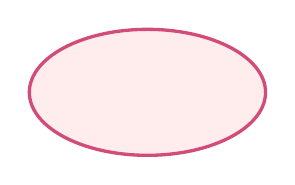
\begin{tikzpicture}
\filldraw[color=purple!70, fill=pink!30, very thick](25mm,25mm) ellipse (15mm and 8mm);
\end{tikzpicture}
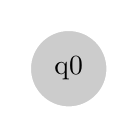
\begin{tikzpicture}
\filldraw[color=white!60, fill=black!20, very thick](10mm,10mm) circle (5mm);
\node at (10mm,10mm) {q0};
\end{tikzpicture}

\begin{tikzpicture}
\filldraw[color=white!60, fill=black!20, very thick](10mm,10mm) circle (5mm);
\node at (10mm,10mm) {};
\end{tikzpicture}
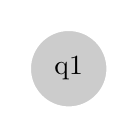
\begin{tikzpicture}
\filldraw[color=white!60, fill=black!20, very thick](10mm,10mm) circle (5mm);
\node at (10mm,10mm) {q1};
\end{tikzpicture}

\begin{tikzpicture}
\filldraw[color=white!60, fill=black!20, very thick](10mm,10mm) circle (5mm);
\filldraw[color=white!60, fill=none, very thick](10mm,10mm) circle (4mm);
\node at (10mm,10mm) {};
\end{tikzpicture}
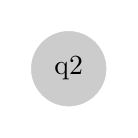
\begin{tikzpicture}
\filldraw[color=white!60, fill=black!20, very thick](10mm,10mm) circle (5mm);
\node at (10mm,10mm) {q2};
\end{tikzpicture}
\end{document}
